\section{Study on neutron capture by hydrogen in the water phase}
\subsection{Selection Criteria and efficiency}
\subsubsection{The selection in the Fast reconstruction}
In the Fast reconstruction, we are going to remove dark noise trigger and some events from the PMT glass.

\paragraph{Before selection}
To evaluate the selection efficiency and the background suppression performance, we defined a cylindrical volume ($\rho$<\SI{1}{m}) centered in the detector, and statistically modeled the signal-to-background ratio.

\begin{figure}[!htbp]
	\centering
	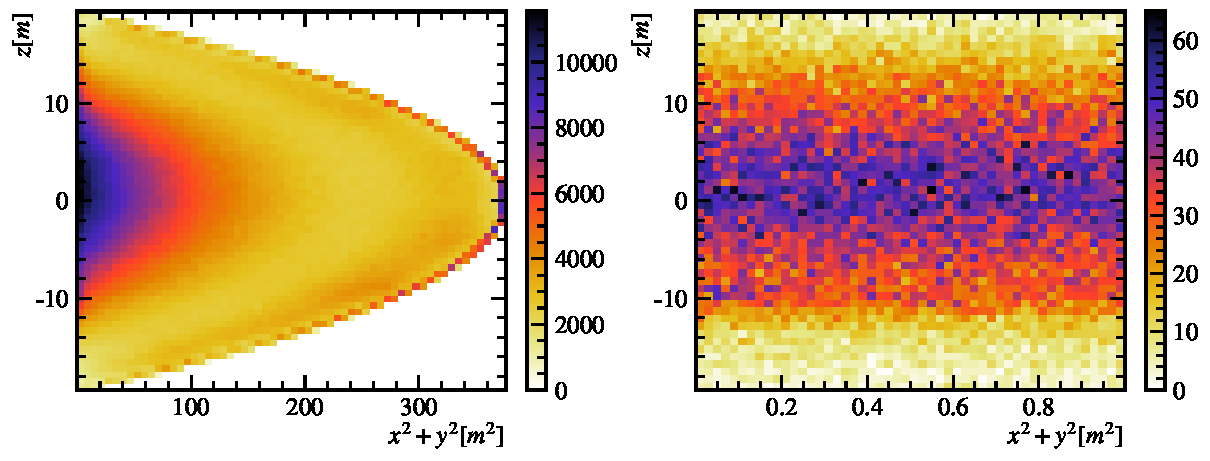
\includegraphics[width=0.7\textwidth]{neutrontag/fastrecon/3671.pdf}
	\caption{The reconstructed position distribution of the Fast reconstruction.}
	\label{fast:all}
\end{figure}

\begin{figure}[!htbp]
	\centering
	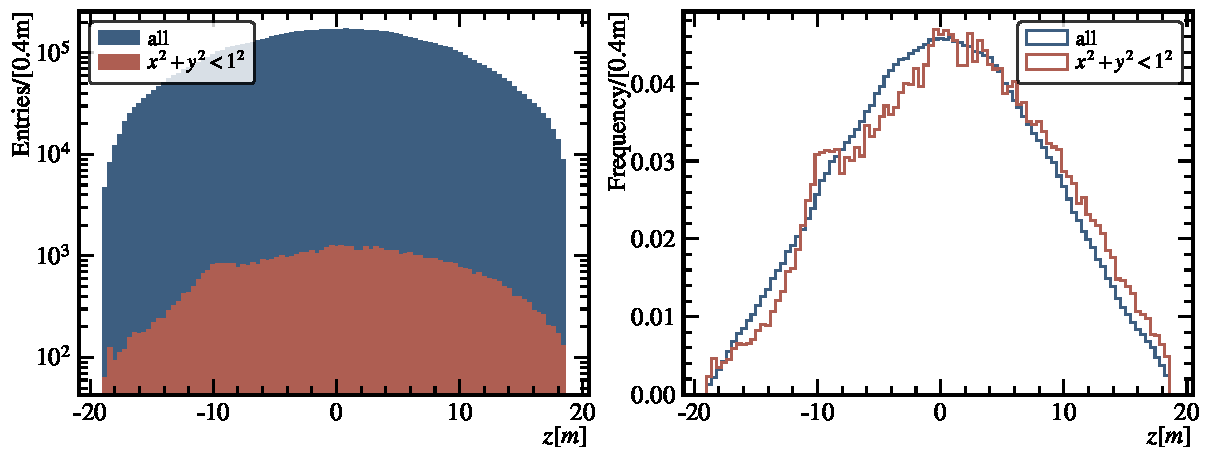
\includegraphics[width=0.7\textwidth]{neutrontag/fastrecon/3671_z.pdf}
	\caption{The reconstructed $z$ distribution of the Fast reconstruction, while $\rho$<\SI{1}{m}}
	\label{fast:z}
\end{figure}


\begin{figure}[!htbp]
	\centering

	\begin{subfigure}[b]{0.4\textwidth}
		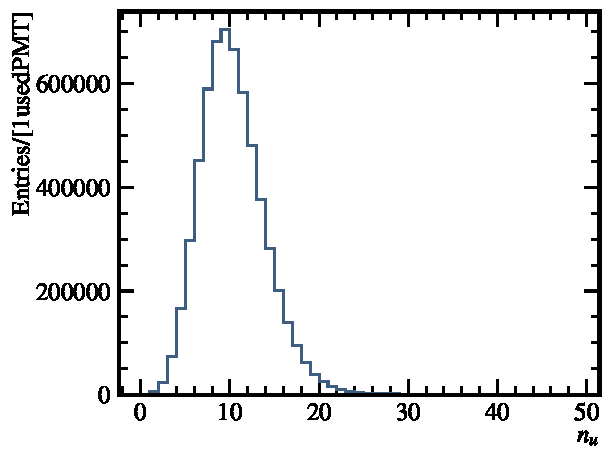
\includegraphics[width=\textwidth]{neutrontag/fastrecon/usedPMT.pdf}
		\caption{Distribution of the number of used PMTs ($n_u$) in the Fast reconstruction.}
		\label{fast:combined:a}
	\end{subfigure}

	\begin{subfigure}[b]{0.4\textwidth}
		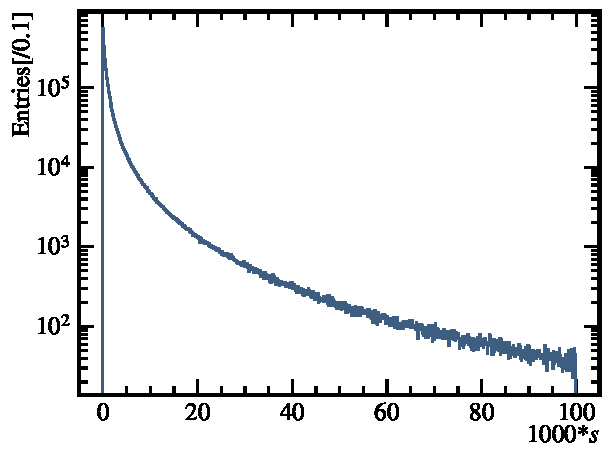
\includegraphics[width=\textwidth]{neutrontag/fastrecon/score.pdf}
		\caption{Distribution of score~($s$) in the Fast reconstruction.}
		\label{fast:combined:b}
	\end{subfigure}

	\caption{Distributions of key parameters in the Fast reconstruction: (a) number of used PMTs ($n_u$), and (b) score~($s$).}
	\label{fast:combined}
\end{figure}

\paragraph{Unknown events}
The z-distribution in Figure \ref{fast:z} displays asymmetry, with excess events in the positive z-region despite the calibration source at $z=-10$\si{m}. A background cut ($n_u>15$) isolates a cluster near $z=10$\si{m}, where events exhibit momentum vectors oriented anti-aligned with the z-axis. We use a cut of $p_z/p>-0.83$ to remove them and the efficiency for events should be $\epsilon_p=91.5$\si{\percent}.
\begin{figure}[!htbp]
	\centering
	\begin{subfigure}[b]{0.4\textwidth}
		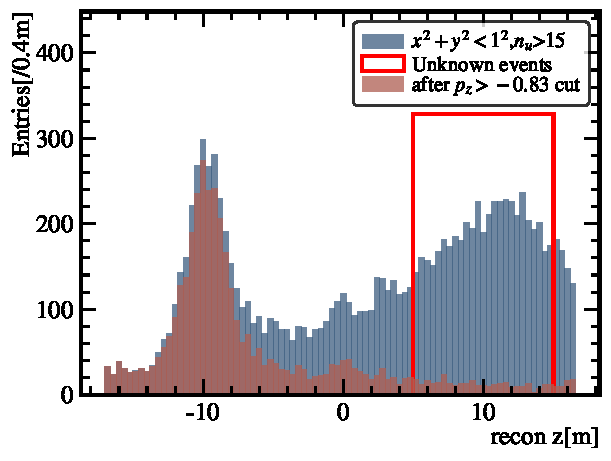
\includegraphics[width=\textwidth]{neutrontag/fastrecon/z_pz.pdf}
		\caption{Distribution of $z$ in the Fast reconstruction before and after the cut of $p_z/p>-0.83$.}
		\label{fast:pzcut}
	\end{subfigure}

	\begin{subfigure}[b]{0.4\textwidth}
		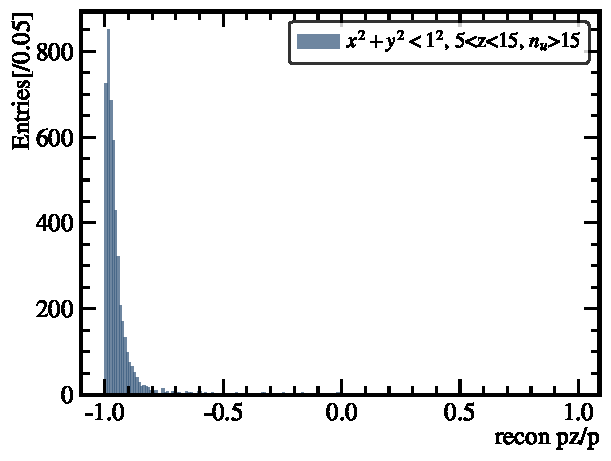
\includegraphics[width=\textwidth]{neutrontag/fastrecon/pz.pdf}
		\caption{Distribution of $p_z/p$ in the Fast reconstruction.}
		\label{fast:pz}
	\end{subfigure}

	\caption{Distributions of key parameters in the Fast reconstruction: (a) number of used PMTs ($n_u$), and (b) score~($s$).}
	\label{fast:pzcombined}
\end{figure}

\paragraph{The selection of $n_u$}
Before selecting events based on the number of $n_u$, $p_z/p>-0.83$ was applied. Under the null hypothesis~(no calibration source), the z-coordinate of background events is modeled as $\mathcal{N} (z \vert \mu_b=0, \sigma_b)$. When the calibration source is active at $z=-10$\si{m}, the signal distribution becomes $\mathcal{N} (z \vert \mu_s=-10, \sigma_s)$. The observed data are therefore fit to a mixture model~(Mix Gauss fit):
\begin{equation}
	f(z)=N_b*\mathcal{N} (z \vert \mu_b=0, \sigma_b)+N_s*\mathcal{N} (z \vert \mu_s=-10, \sigma_s)
	\label{eq:2g}
\end{equation}
By calculating the ratio of $N_s$ with different cuts to that without cuts, the select efficiency can be roughly estimated. The background rejection ratio can be determined by computing the ratio of $N_b$ to the value without cut. Additionally, the signal-to-noise ratio can be approximately estimated using $N_s/\sqrt{N_b}$. From Figure~\ref{fast:nucut}, $N_{b0}=20332\pm211, N_{s0}=1026\pm114$.
\begin{figure}[!htbp]
	\centering
	\begin{subfigure}[b]{0.4\textwidth}
		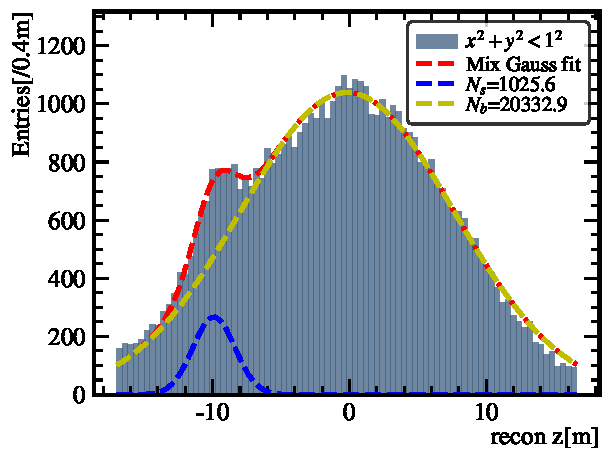
\includegraphics[width=\textwidth]{neutrontag/fastrecon/z_origin.pdf}
		\caption{The fit result of $z$ without cut of $n_u$ after the cut of $x^2+y^2<1, p_z/p>-0.83$.}
		\label{fast:nonucut}
	\end{subfigure}

	\begin{subfigure}[b]{0.4\textwidth}
		\includegraphics[page=8, width=\textwidth]{neutrontag/fastrecon/npmtCut.pdf}
		\caption{The fit result of $z$ after the cut of $n_u>8$}
		\label{fast:exnucut}
	\end{subfigure}
	\caption{Distributions of $z$ before and after the cut of $n_u$.}
	\label{fast:nucut}
\end{figure}

From the Figure~\ref{fast:nusummary}, as the selection of $n_u$ increases, $N_s$ gradually decreases, while the $N_s/\sqrt{N_b}$ progressively improves. Ultimately, balancing the data volume and the number of signal events, the cut $n_u$ > 8 was selected, with an estimated efficiency of  $\epsilon_{n_u}=69.24\pm10.6$\si{\percent}.

\begin{figure}[!htbp]
	\centering
	\begin{subfigure}[b]{0.4\textwidth}
		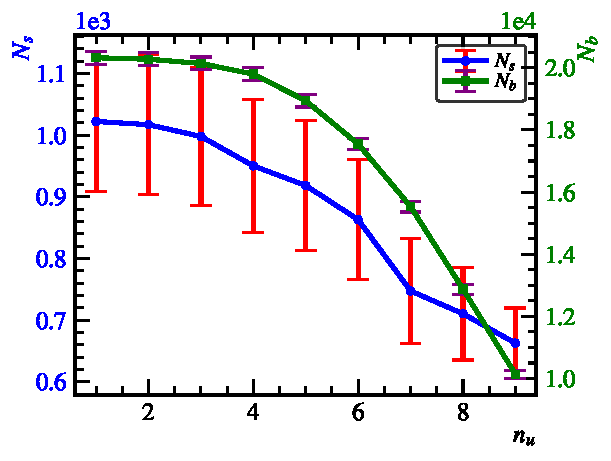
\includegraphics[width=\textwidth]{neutrontag/fastrecon/npmtNsNb.pdf}
		\caption{$N_s$ and $N_b$}
		\label{fast:nuNsNb}
	\end{subfigure}

	\begin{subfigure}[b]{0.4\textwidth}
		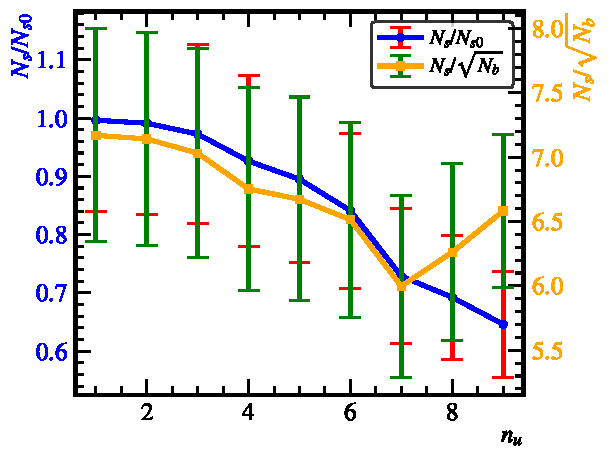
\includegraphics[width=\textwidth]{neutrontag/fastrecon/npmtNssn.pdf}
		\caption{$N_s/N_{s0}$ and $N_s/\sqrt{N_b}$}
		\label{fast:nuSN}
	\end{subfigure}
	\caption{The result of the different cut of $n_u$.}
	\label{fast:nusummary}
\end{figure}

\paragraph{The selection of $s$}
We also use the mixture model in the selection of $s$.
\begin{figure}[!htbp]
	\centering
	\begin{subfigure}[b]{0.4\textwidth}
		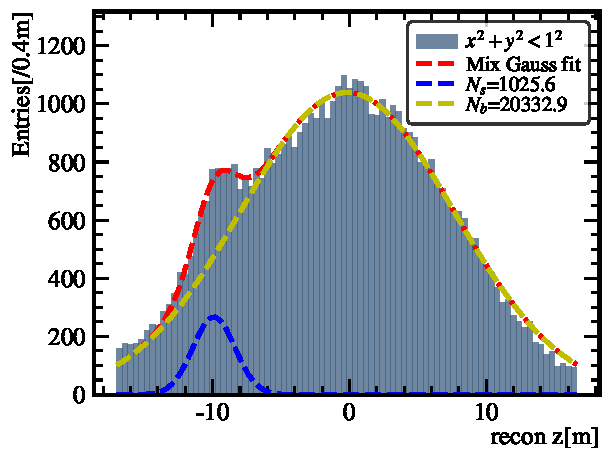
\includegraphics[width=\textwidth]{neutrontag/fastrecon/z_origin.pdf}
		\caption{The fit result of $z$ without cut of $s$ after the cut of $x^2+y^2<1, p_z/p>-0.83$.}
		\label{fast:snucut}
	\end{subfigure}

	\begin{subfigure}[b]{0.4\textwidth}
		\includegraphics[page=6, width=\textwidth]{neutrontag/fastrecon/scoreCut.pdf}
		\caption{The fit result of $z$ after the cut of $s>0.0016$}
		\label{fast:exscut}
	\end{subfigure}
	\caption{Distributions of $z$ before and after the cut of $s$.}
	\label{fast:scut}
\end{figure}

From the Figure~\ref{fast:ssummary}, as the selection of $s$ increases, $N_s$ changes a little, while $N_b$ decreases a lot, and the $N_s/\sqrt{N_b}$ progressively improves. Ultimately, the cut $s$ > 0.0016 was selected, with an estimated efficiency of  $\epsilon_{s}=71.4\pm8.6$\si{\percent}.
\begin{figure}[!htbp]
	\centering
	\begin{subfigure}{0.4\textwidth}
		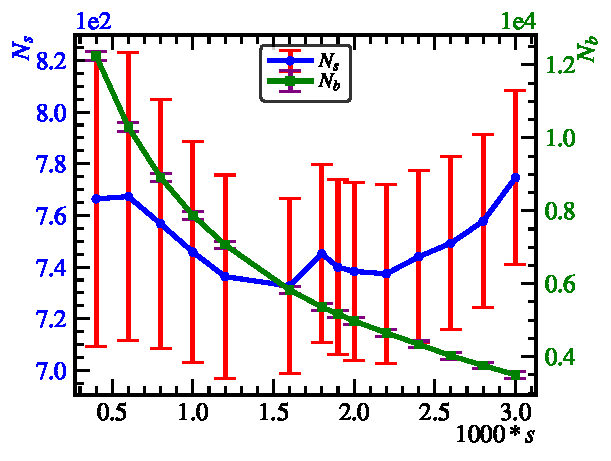
\includegraphics[width=\textwidth]{neutrontag/fastrecon/scoreNsNb.pdf}
		\caption{$N_s$ and $N_b$}
		\label{fast:sNsNb}
	\end{subfigure}

	\begin{subfigure}{0.4\textwidth}
		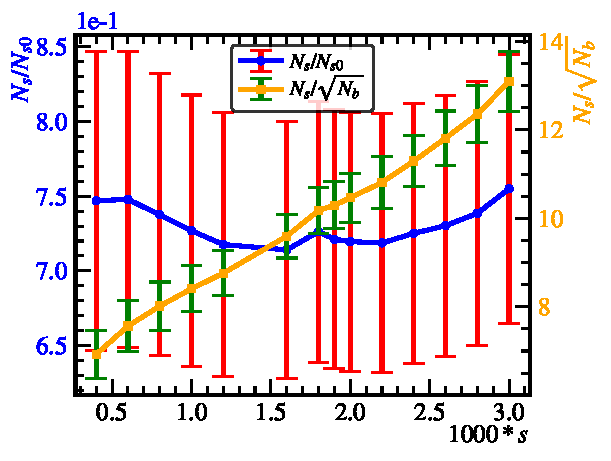
\includegraphics[width=\textwidth]{neutrontag/fastrecon/scoreNssn.pdf}
		\caption{$N_s/N_{s0}$ and $N_s/\sqrt{N_b}$}
		\label{fast:sSN}
	\end{subfigure}
	\caption{The result of the different cut of $s$.}
	\label{fast:ssummary}
\end{figure}

\paragraph{The selection of events inputted to likelihood-based reconstruction }
To improve the vertex and energy resolution, the selected events are fed into a likelihood-based reconstruction algorithm.
The selection criterias:
\begin{itemize}
	\item $n_u>5$
	\item $s>0.002$
	\item $x^2+y^2+z^2<16.8^2$
\end{itemize}

And the selection efficiency is $\epsilon_f=74.0\pm8.9$\si{\percent}.
\begin{figure}[!htbp]
	\centering
	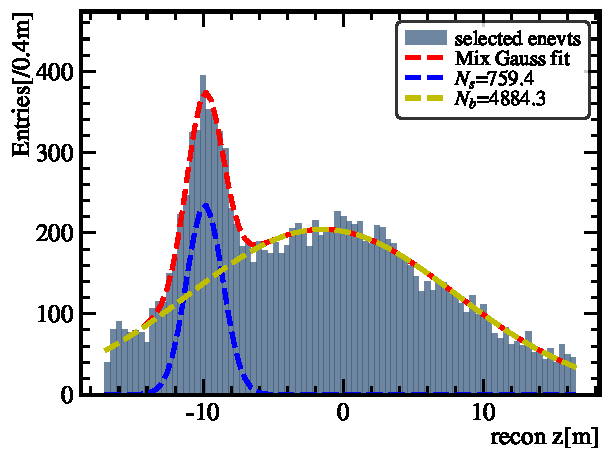
\includegraphics[width=0.5\textwidth]{neutrontag/fastrecon/z_input.pdf}
	\caption{The selected events after selection}
	\label{fast:input}
\end{figure}

\subsubsection{The selection in the likelihood-based reconstruction algorithm}
After the cuts:
\begin{itemize}
	\item $x^2+y^2+z^2<17^2$
	\item $p_z/p>-0.83$
	\item $k>-0.85$
	\item $n_{10}-n_{b}>15$
	\item $n_c>8$
\end{itemize}
\begin{figure}[!htbp]
	\centering
	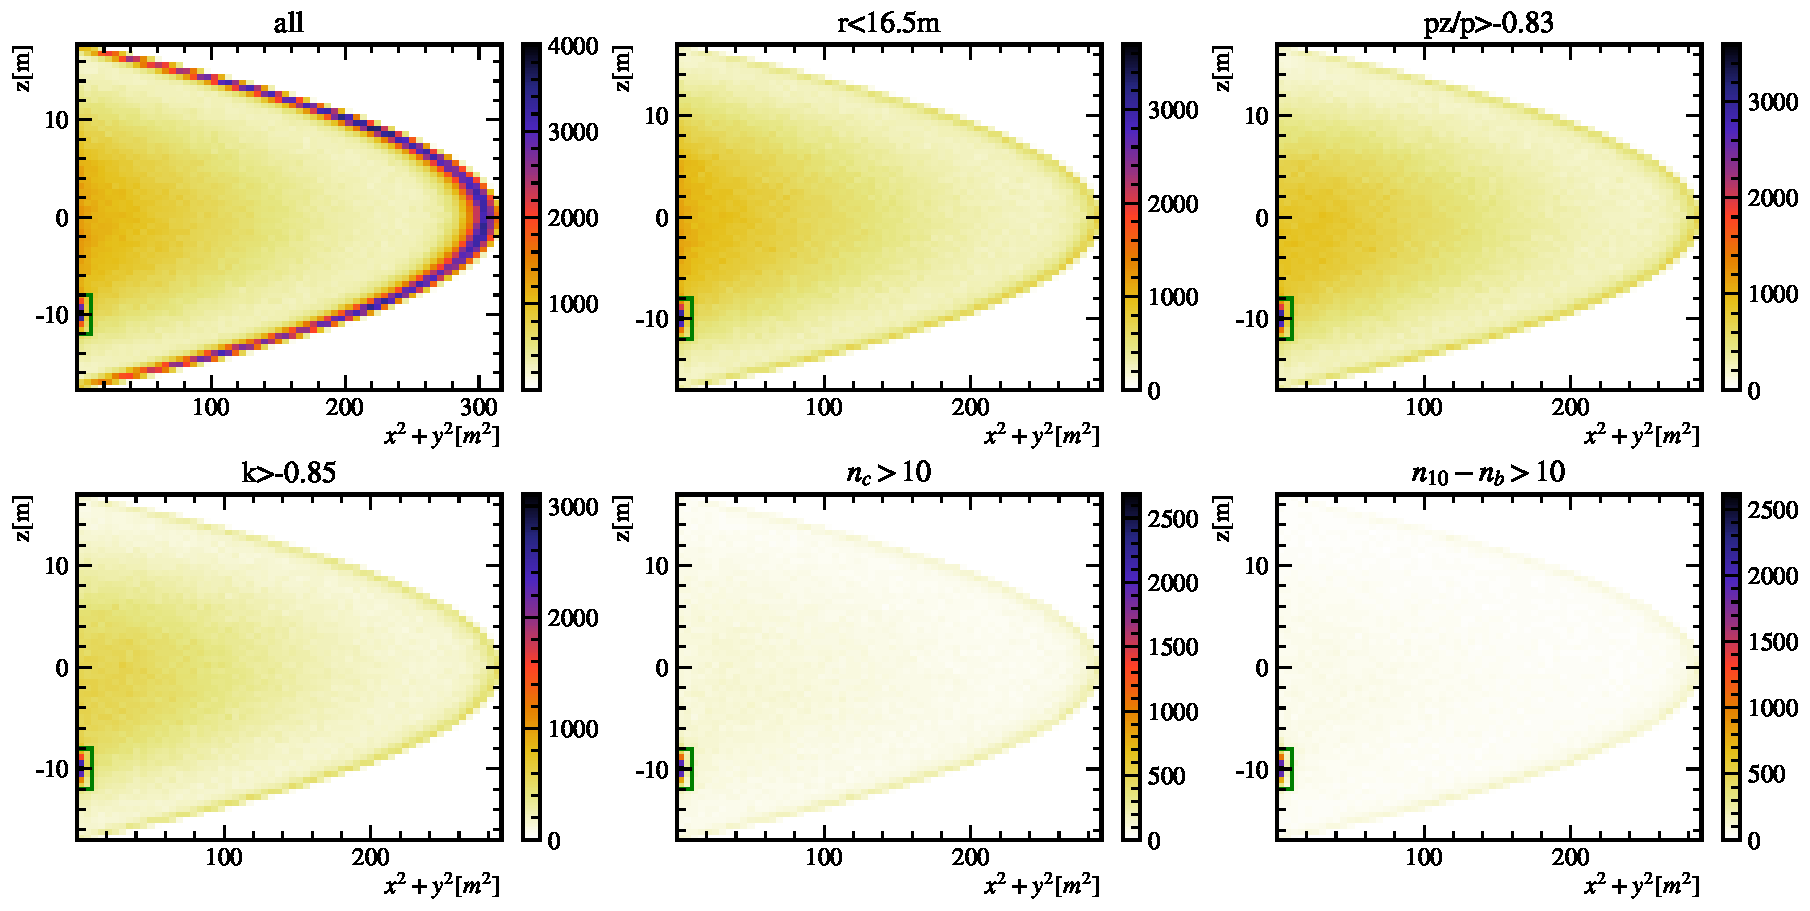
\includegraphics[width=0.9\textwidth]{neutrontag/lb/3671.pdf}
	\caption{The position distribution of the likelihood-based reconstruction.}
	\label{lb:pos}
\end{figure}

\paragraph{The distribution of $z$}
\begin{figure}[!htbp]
	\centering
	\begin{subfigure}{0.4\textwidth}
		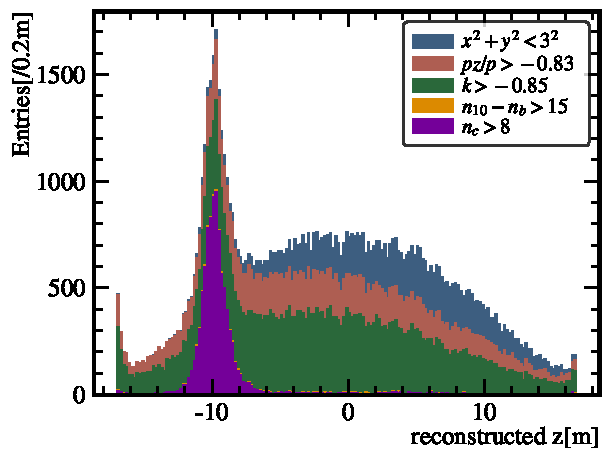
\includegraphics[width=\textwidth]{neutrontag/lb/3671_z.pdf}
		\caption{}
		\label{lb:sNsNb}
	\end{subfigure}

	\begin{subfigure}{0.4\textwidth}
		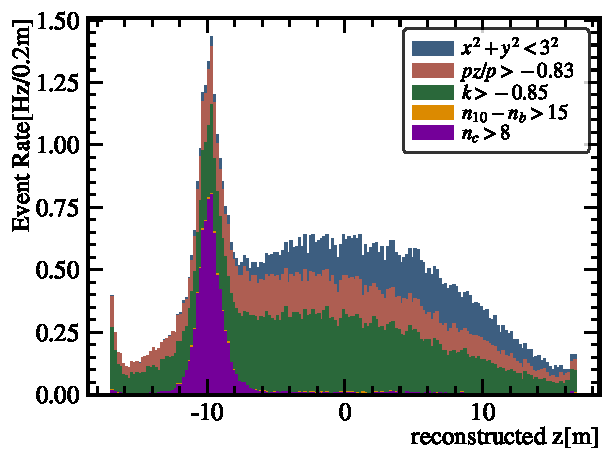
\includegraphics[width=\textwidth]{neutrontag/lb/3671_z_rate.pdf}
		\caption{}
		\label{lb:sSN}
	\end{subfigure}
	\caption{The distribution of $z$ after a cut of $x^2+y^2<3^2$.}
	\label{lb:ssummary}
\end{figure}

\subsection{The tag efficiency of n-H capture}
\paragraph{Without the position truth cut}
After the cuts, the number of remained events is 8573.
Coincident Criteria:
\begin{itemize}
	\item $dR$<\SI{5}{m}
	\item {for prompt signal:
	      \begin{itemize}
		      \item $n_{10}-n_{b}>15$
		      \item $n_c>8$
	      \end{itemize}
	      }
	\item {for delayed signal:
	      \begin{itemize}
		      \item $n_{10}-n_{b}>5$
		      \item $p<6$\si{MeV}
	      \end{itemize}}
	\item $1<dt<1500$\si{us}
	\item $(n_{10}-n_{b})_p-(n_{10}-n_{b})_d>2$
\end{itemize}

About 391 pairs are selected, the efficiency is \SI{4.6}{\percent}.
\begin{figure}[!htbp]
	\centering
	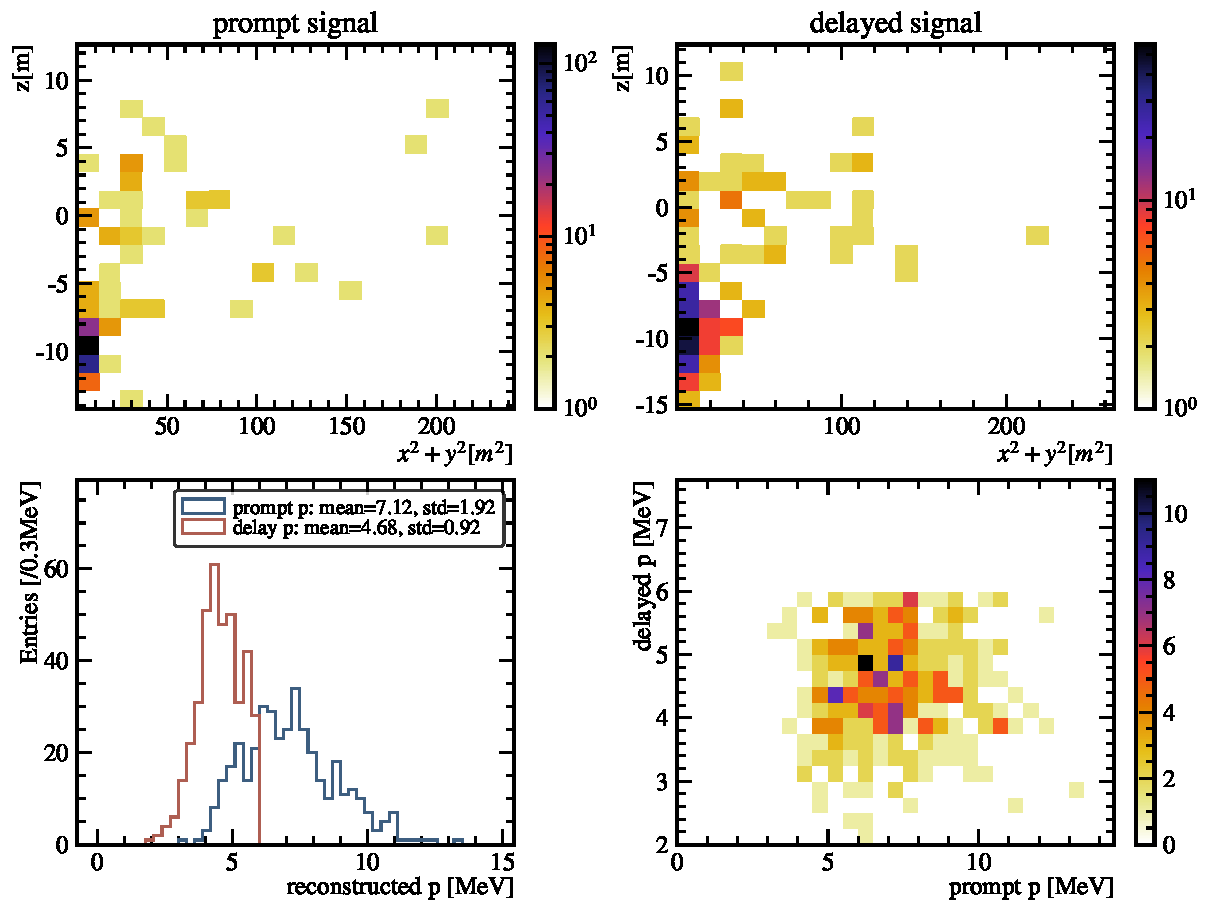
\includegraphics[width=0.9\textwidth]{neutrontag/coin/3671_coin.pdf}
	\caption{The distribution of prompt and delayed signals.}
	\label{coin:pos0}
\end{figure}

\begin{figure}[!htbp]
	\centering
	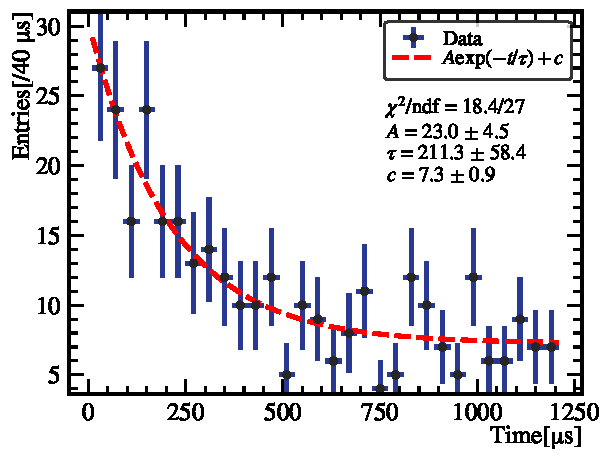
\includegraphics[width=0.5\textwidth]{neutrontag/coin/3671_coin_fit.pdf}
	\caption{The $dt$ fit}
	\label{coin:dt0}
\end{figure}

\paragraph{With the postion truth cut}
Additional cut:
\begin{itemize}
	\item For prompt signal: $x^2+y^2+(z+10)^2<4^2$
	\item For delayed signal: $x^2+y^2+(z+10)^2<6^2$
\end{itemize}

About 221 pairs are selected, the efficiency is \SI{2.6}{\percent}.
\begin{figure}[!htbp]
	\centering
	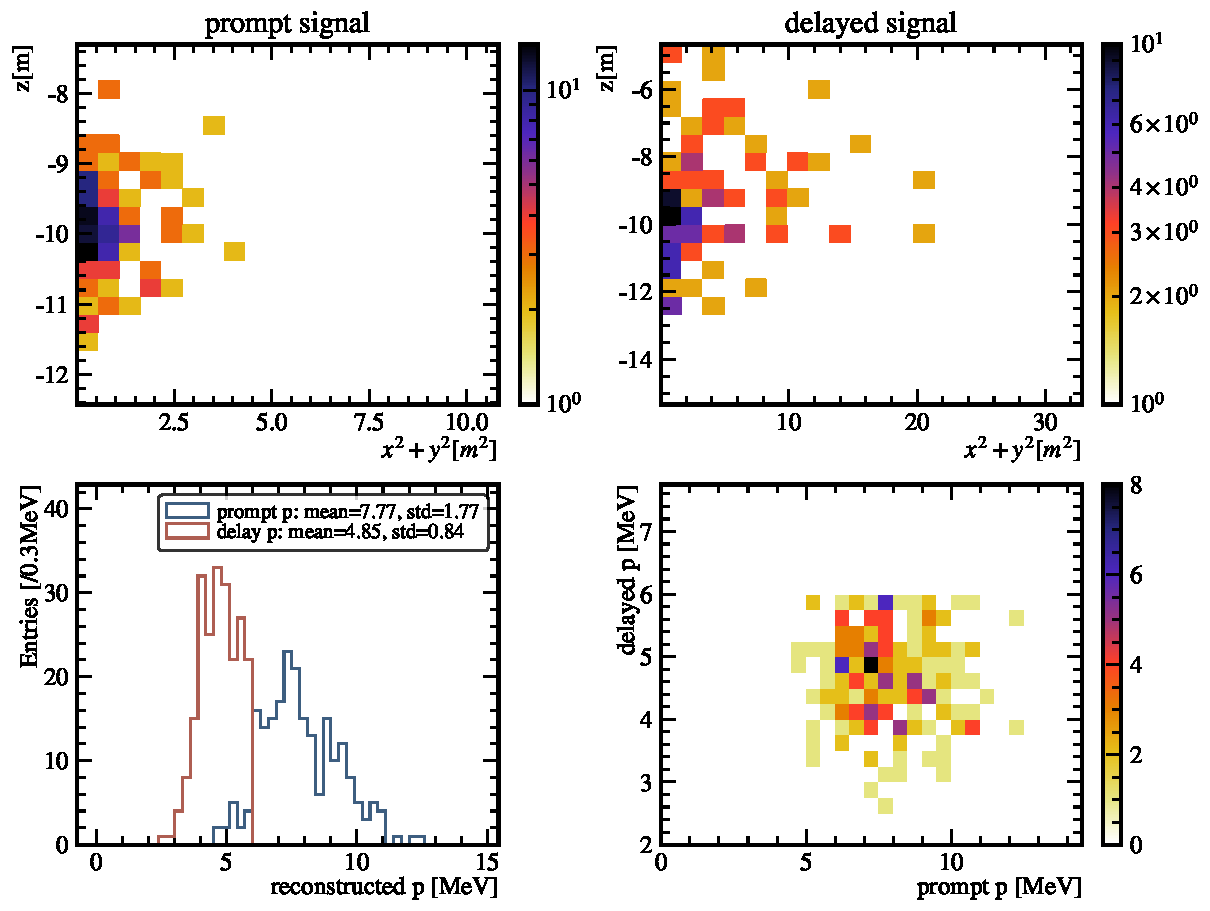
\includegraphics[width=0.9\textwidth]{neutrontag/coin/3671_pos_coin.pdf}
	\caption{The distribution of prompt and delayed signals.}
	\label{coin:pos1}
\end{figure}

\begin{figure}[!htbp]
	\centering
	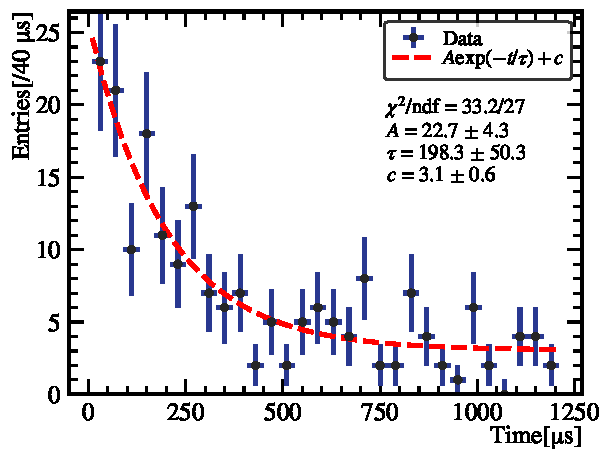
\includegraphics[width=0.5\textwidth]{neutrontag/coin/3671_coin_pos_fit.pdf}
	\caption{The $dt$ fit}
	\label{coin:dt1}
\end{figure}

Before and after applying the truth-based cut, the fit of dt shows that the signal component $A$ remains nearly unchanged, while the accidental coincidence background $c$ is significantly reduced.
